%----------------------------------------------------------------------------
\chapter{\bevezetes}
%----------------------------------------------------------------------------
\label{ch:bev}
\selecthungarian

\section{A dolgozat célja és felépítése }
A modern informatika egyik fontos és feltörekvő területe az IT Security, amely a számítógép ipar fejlődésével egyre nagyobb szerepet kap. Ahogy a gépek számító kapacitása növekszik, egyre könnyebben megoldhatók olyan problémák, amelyek addig lehetetlennek, elfogadható időben kivitelezhetetlennek tűntek. Ez a fejlődés az egész szektort arra készteti, hogy folyamatosan fejlődjön, a meglévő alkalmazásokat, módszereket, algoritmusokat javítsa. Emellett a modern világban egyre nagyobb vállalatok jönnek létre, amelyeknek egyre nagyobb személyzetre van szükségük a működéshez, ami indokolttá teszi egy megfelelően stabil és jól kezelhető informatikai támogató réteg kialakítását. Több ezer, akár több tízezer alkalmazott mellett gyorsan átláthatatlanná válik, hogy kinek milyen eszközökhöz, akár hardveres, akár szoftvereshez van hozzáférése, ezek egyesével való beállítása és karbantartása pedig emberi léptékkel mérve szinte kivitelezhetetlen, és rendkívül költséges a fent említett támogató szoftverek nélkül.

 Jelen dolgozat az IT Security világának számos területéből kettővel foglalkozik, ennek a kettőnek is elsősorban a kapcsolatával. Az egyik terület a Security Information and Event Management (SIEM), ami egy informatikai rendszer biztonsági felügyeletével foglalkozik. A másik terület az Identity management (IdM), ami pedig az alkalmazottak és a hozzájuk tartozó jogosultságok életciklusának menedzselésével foglalkozik. A cél a kettő terület összekapcsolása oly módon, hogy az IdM szoftverben található hasznos, felhasználókkal kapcsolatos adatok elérhetők legyenek a SIEM szoftver számára. Ezek olyan kontextust szolgáltatnak, amely az elemi eseményekből nem következik. Például a SIEM által feldolgozott események jellemzően köthetők egy felhasználónévhez, viszont nem állnak rendelkezésre azok az információk, hogy az adott felhasználónév mely valós személyhez tartozik és az illető esetleg kiléptetés alatt áll-e, a biztonsági házirenddel összhangban van-e egy adott fiók létezése és jogosultsági szintje, vagy hogy mikor és ki hagyta jóvá a felhasználói fiók létrehozását. Mindezen adatok az IdM rendszerből kinyerhetők. Az integráció célja, hogy az IdM rendszerben tárolt releváns adatokkal tudjuk támogatni a SIEM szabályrendszerét. \cite{whatisidm}

Egy ilyen integrációval az alábbiak, valamint ehhez hasonló use-case-ek valósíthatók meg:

\begin{itemize}
	\item Inaktív személyekhez tartozó felhasználói fiókok - Ez az információ hasznos lehet egy QRadar szabályhoz például olyan esetben, ha arra vagyunk kíváncsiak, hogy volt-e aktivitás olyan fiókkal, amelynek a tulajdonosa már nem a cég alkalmazottja, és a fióknak meg kellett volna szűnnie.
	
	\item Valós személyhez nem köthető felhasználói fiókok - Ezek az árva fiókok biztonsági kockázatokat jelenthetnek, mert a hozzájuk tartozó műveletekért nincs kit felelősségre vonni. Ezért hasznos lehet egy olyan QRadar szabály, ami kifejezetten az ilyen esetekben jelez.
	
	\item Adott erőforráshoz legitim hozzáféréssel rendelkező személyek - Ez az információ olyan esetben lehet hasznos, ha például egy támadás kiinduló pontjaként sikerül azonosítani egy eszközt. Ezzel lehetséges az olyan felhasználói fiókkal történő aktivitás észlelése, amelyet az IdM szabályrendszerét megkerülve hoztak létre.
\end{itemize}

A diplomatervem keretében fejlesztettem egy integrációs modult, amely egy általános célú adatszinkronizációs eszköz az IdM és a SIEM rendszer között, valamint ennek segítségével megvalósítottam a fent leírt use-case-ekhez szükséges lekérdezéseket és adatszinkronizációt.

A SIEM számára nemcsak a felhasználókkal kapcsolatos adatok, hanem a jogosultságkezeléssel kapcsolatos folyamatok eseményei is relevánsak, amelyeknek szintén az IdM rendszer a forrása. A diplomatervem során megvalósítottam egy olyan eszközt, amely bővíti a SIEM számára látható IdM események körét, ezzel teljesebbé téve az IdM rendszer biztonsági monitorozását.

A dolgozat felépítése a következő:

\begin{itemize}
	\item Az \ref{ch:bev}. fejezet a dolgozat valamint a diplomaterv célját definiálja és járja körbe, rövid bemutatót adva a felhasznált technológiák főbb tulajdonságairól.
	
	\item A \ref{ch:tech}. fejezet a projektben megismert és felhasznált technológiákat mutatja be, kitérve a feladat számára fontos technológiákra.
	
	\item A \ref{ch:imp}. fejezet a konkrét implementációs kérdéseket, valamint az ezekre adott megoldásaimat mutatja be.
	
	\item A \ref{ch:usage}. fejezet az elkészült megoldások telepítését és használatát mutatja be.
	
	\item A \ref{ch:sum}. fejezet egy rövid összefoglaló a féléves munkámról.
	
\end{itemize}

\section{Security Information and Event Management}

A Security Information and Event Management az informatikai rendszer részeinek monitorozásával foglalkozik biztonsági szempontból. Az infrastruktúrában található eszközök által generált eseményekhez hozzáfér a SIEM megoldás, és ez végzi az események feldolgozását és elemzését. A monitorozott rendszerek működésükkel kapcsolatos információkat biztosítanak a SIEM irányába valamilyen formában, általában log sorokként. A SIEM szerver ezeket feldolgozza, és a szabályrendszerének megfelelő eseményekből úgynevezett biztonsági incidenseket hoz létre, akár egyéb forrásokból érkező plusz információk felhasználásával. Ilyen egyéb forrás lehet hálózati forgalom, valamilyen adatbázisból lekért adatok, vagy előre definiált, a szerverre feltöltött adatok. 

Nem triviális feladat a szabályrendszert úgy konfigurálni, hogy a fals pozitív riasztások száma alacsony maradjon, miközben a valós támadásokat hatékonyan detektálja. 

A megvalósítandó integráció a szabályrendszer hatékonyságát kétféleképpen segíti elő. Egyrészt, az IdM-ben redelkezésre álló információk segítségével olyan támadásminták detekciója válik lehetővé, amelyeket enélkül a SIEM nem lenne képes észlelni. Másrészt, a SIEM szabályrendszerét aktuális adatokkal látja el, amely a fals pozitív riasztások számát képes csökkenteni.

Emellett az általam generált és feldolgozott IdM-ből érkező jogosultsági folyamatok eseményein keresztül a SIEM további, fontos incidenseket képes detektálni.

Jelen feladatnak nem célja a SIEM szabályrendszerének részletes kidolgozása, a dolgozat témája az IdM és a SIEM közötti adatszinkronizáció lehetőségének megteremtése.

\section{Identity management}

Az Identity management a fejlődő nagyvállalatok fent említett problémáiból a nagyszámú alkalmazott hozzáféréseinek kezelését és a dolgozók, mint informatikai entitások életciklusának menedzselését oldja meg. Ez magában foglalja az entitások  rendszerezését, csoportokhoz rendelését, valamint a saját és örökölt jogaik érvényre juttatását.

Minden alkalmazotthoz tartozik egy rekord, amely leírja az adott ember személyes adatait és egyéb olyan információkat, amelyek szükségesek az alkalmazott jogosultságainak meghatározásához. Ezt a létrejött entitást beosztja a megadott információk szerint a megfelelő, előre definiált szerepkörökbe, amely alapján az jogokat kap bizonyos eszközök használatára. Ezen eszközök is entitásként vannak felvéve a rendszerbe, oly módon, hogy elérhetők az eszközhöz (akár szoftveres akár hardveres) tartozó információk és menedzselhető a hozzáférés.

A dolgozat célja ezen alkalmazotti és a hozzájuk kapcsolódó életciklus információinak kinyerése és eljuttatása a SIEM rendszer számára, mivel ezek az információk értékesek lehetnek a biztonsági incidensek kiértékelése szempontjából.

\section{A feladat specifikálása}

Jelen dolgozat feladata egy olyan megoldás fejlesztése, mely lehetővé teszi a fent említett technológiák közti integrációt és az adatszinkronizációt. Az integrációt a IBM által kínált IdM (IBM Security Identity Manager - ISIM\footnote{Lásd \ref{subsec:ISIM} \nameref{subsec:ISIM}}) és SIEM (IBM Security QRadar SIEM - QRadar\footnote{Lásd \ref{subsec:qradar} \nameref{subsec:qradar}}) között dolgoztam ki.
 
A végső megoldás két részből áll, egyrészt egy teljesen új funkcionalitást biztosító integrációs modulból, valamint egy már meglévő funkcionalitást bővítő kiegészítésből. Erre a feladatra eddig nem volt automatikus megoldás, ezért ez a projekt ezt a hiányt hivatott betölteni.

A QRadarban már megtalálható egy olyan modul, ami képes az ISIM-ben generált események egy részhalmazának feldolgozására és értelmezésére, de ez csak bizonyos audit események feldolgozására képes. Ezt kibővítendő készítettem egy megoldást, amely az előző funkcionalitást egészíti ki egyéb, eddig nem feldolgozott eseményekkel, amelyek plusz információt hordoznak biztonsági szempontból. A modulhoz használt keretrendszert a TDI \footnote{\label{foot:TDI}Lásd \ref{subsec:TDI} \nameref{subsec:TDI}} nyújtja.

Mindkét integráció megvalósításához a Java alapú technológiát választottuk. A döntést indokolja, hogy jól illeszkedik a tipikus nagyvállalati környezethez, az IBM kiterjedt tapasztalattal és eszközkészlettel rendelkezik ezen a téren, valamint ez az ISIM technológiája és programozói interfésze is.

Az integráció megvalósításának első lépése egy Java API fejlesztése a QRadar-hoz. A QRadar egy technológiafüggetlen REST API-val rendelkezik. Ahhoz, hogy Java alkalmazásból az API számunkra fontos része használható legyen, egy Java Wrapper library-t fejlesztettem, amely Java metódusok formájában teszi lehetővé a QRadar API használatát. Ez a wrapper egy általános megoldást ad a QRadarba feltöltött adatok (lsd. \ref{lbl:reference_data}) lekérésére és módosítására, így egy később felmerülő projektben is hasznos lehet.

Az integráció megvalósítására két architektúrát is kidolgoztunk, amelyeket a következő két alfejezetben ismertetek.

\subsection{Integráció TDI segítségével}

A Tivoli Directory Integrator (TDI \footnote{\label{foot:TDI}Lásd \ref{subsec:TDI} \nameref{subsec:TDI}}) egy gyakran használt, általános célú integrációs eszköz. 
A TDI segítségével különböző adatforrásokat, amelyek más-más protokollon keresztül érhetők el, és más-más formátumban és struktúrában tárolják az adatokat, egy egységes ú.n.~Connector interfészen keresztül érhetjük el. Az adattranszformációs feladatokat ú.n.~assembly line formájában valósíthatjuk meg a TDI grafikus felületén. Egy assembly line egy műveletsort definiál, amely során felhasználhatjuk a connectorokat adat olvasásra, keresésre, kiírásra, valamint Javascript segítségével tetszőleges adattranszformációt valósíthatunk meg. A megfelelő protokoll és parser kiválasztásáról a használt connector gondoskodik, így az assembly line kompakt módon csak a valódi adattranszformációt definiálja. 

A TDI gyári connector készletét kiegészítettem egy új, saját fejlesztésű connectorral, amely a fent említett wrapper könyvtár segítségével képes reference data-kat feltölteni és lekérni a QRadartól. A hálózati erőforrások hatékony használatának céljából a connector külön akkumulálja a feltöltendő adatokat, és a futása végén, egyben tölti azokat fel. Az általam létrehozott connector egy általános célú TDI connector, így szabadon újra felhasználható nem csak az ISIM-mel való integrációra, hanem tetszőleges TDI assembly line formájában megvalósított integrációs feladatra. 

Ebben a megvalósításban a QRadar és az ISIM közti integrációt TDI assembly line-ok formájában valósítottam meg, melyeket a TDI által biztosított szerver komponens dolgoz fel és futtat. A TDI gyári funkcióit és grafikus interfészét felhasználva az egyes assembly line-ok fejlesztése időtakarékos és költséghatékony. Ennek a megvalósításnak hátránya, hogy a megoldások a TDI-hez kötöttek, valamint a lehetőségeknek határt szabnak a TDI által nyújtott lehetőségek. Egy újabb lekérdezés vagy lekérdezéstípus konfigurálása, ütemezése a TDI fejlesztői felületén történik, így az üzemeltetési feladatok ellátásához a TDI ismerete szükséges.


\begin{figure}[]
	\centering
	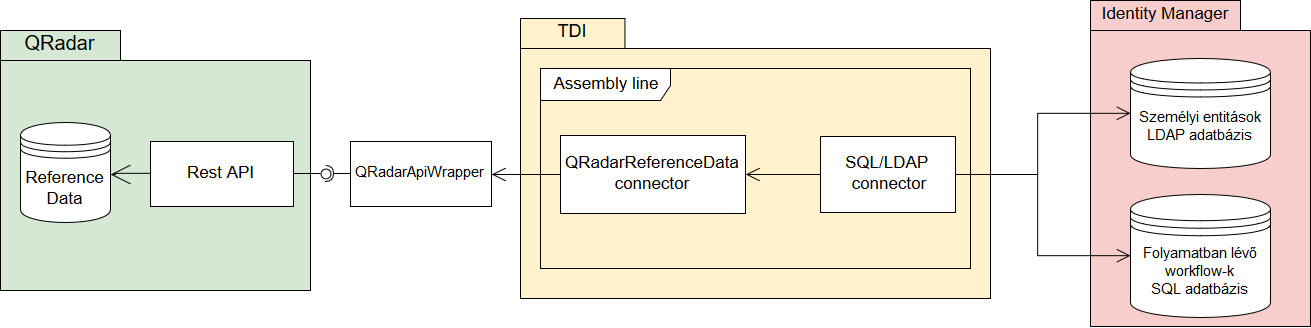
\includegraphics[width=1.0\linewidth]{figures/TDI_architecture.png}
	\caption{Architektúra TDI esetén}
	\label{fig:tdi-architecture}
	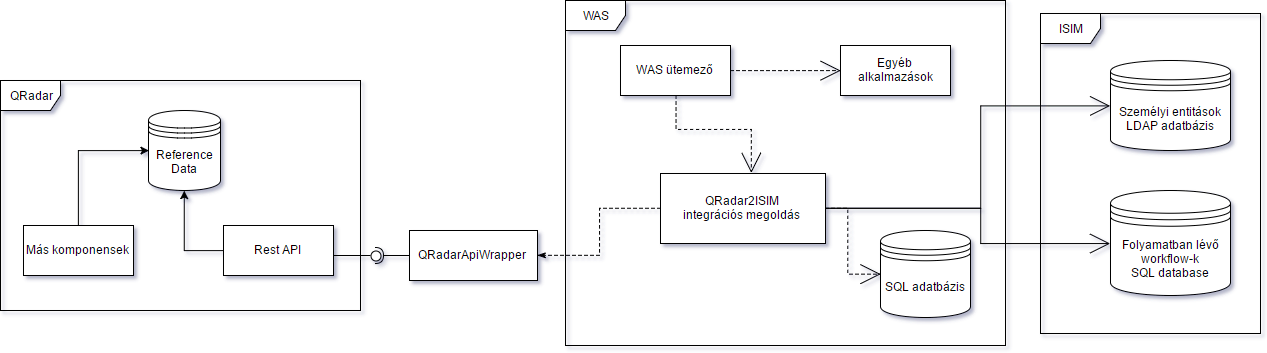
\includegraphics[width=1.0\linewidth]{figures/WAS_architecture.png}
	\caption{Architektúra WAS esetén}
	\label{fig:wasarchitecture}
\end{figure}


\subsection{Integráció webes (WAS) alkalmazás formájában}

Ennél a megoldásnál egy IBM WebSphere Application Server (WAS) környezetre fejlesztett alkalmazást készítettünk egy projekt keretében, amely a QRadarral való kommunikációra felhasználja az általam fejlesztett wrapper-t. Az alkalmazás rendelkezik egy felhasználóbarát webes felülettel, melyen keresztül létrehozhatunk és felkonfigurálhatunk szinkronizációs feladatokat. Az integrációt olyan szinkronizációs feladatok valósítják meg, melyek ütemezett futtatására támogatást biztosít az alkalmazás a WAS által nyújtott lehetőségeken keresztül. A feladatok eltárolják az aktuálisan lekérdezett adatokat egy SQL adatbázisba, valamint karbantartanak egy másik táblát ami mindig a QRadarra aktuálisan sikeresen felszinkronizált adatokat tartja számon. Ezen adatbázisok segítségével számolható egy különbség, ami az elégségesen felküldendő adatokat tartalmazza. Ezzel csökkenthető a QRadar irányába a tranzakciónkénti overhead. Emellett ha az alkalmazás inkonzisztenciát érzékel a lokális állapot és a QRadarban megtalálható adatok között, akkor egy teljes szinkronizációval minden adatot felküld, ezzel egy új, konzisztens állapotba állítva a rendszert.

%Ebben a megvalósításban TDI alapú megoldáshoz képest előny, hogy az integrációs adatokhoz tartozó szinkronizáció pontos implementációja saját fejlesztésű, így hozzáigazítható a pontos igényekhez. 
Ebben a megvalósításban a TDI alapú megoldáshoz képest előny, hogy a WAS egy menedzselt környezetet biztosít a futtatáshoz, így jobban felügyelhetők az egyes feladatok, valamint igény szerint könnyen megvalósítható az elosztott, klaszteren futó, hibatűrő működés is. Előny továbbá, hogy saját grafikus felhasználói felülettel rendelkezik, amelyen az üzemeltetési feladatok könnyen elvégezhetők. Új lekérdezéstípus létrehozása Java fejlesztői ismeretet követel meg, konkrét technológiához kötött (pl.~TDI) tudás nem szükséges. A WAS minden ISIM környezetben elérhető, ezért nem szükséges új komponensek telepítése az modul használatához.

A TDI-t használó megoldással szemben a hátránya, hogy a megoldás ISIM specifikus, más forrásokkal való integrációhoz szükség van a forráskód módosítására.
